\documentclass[10pt,twoside,draft]{book}
\usepackage{../../thesis}
\graphicspath{ {../../images/} }

\begin{document}

\chapter{The Logistic Map}
%\addcontentsline{toc}{chapter}{Introduction}
%\chaptermark{Introduction}
%\markboth{Introduction}{Introduction}
\label{chap:intro}
As mentioned in the preliminaries, the exposition focuses on topological dynamical systems.
In particular, we are interested in those that are \textit{chaotic}.
To illustrate what it means to be a system to be chaotic, we study the logistic map.
We do not formally define what it means for a system to be chaotic.
%In fact, we never will.
%We instead look for a definition of chaos that makes sense through studying different definitions and examples.
The present chapter aims to develop intuitive ideas of how chaos should be defined, while we let go of mathematical rigor until the next chapter.
%Next, we proceed to the historical the origin of chaos.
%At last, I discuss how we will go about defining the term 'chaos.'
%An approximation of a differential equation, which is how we treat $L_\mu$ in the current section, is one way to think about some topological dynamical systems.
%However, this characterization of a topological dynamical system fails for most systems that we will see, since we do not require our mappings to be differentiable.

%For the time being, our definition of "chaos" is this: a map that's complicated.
%%%

The logistic map $L_\mu$ is defined as 
\begin{equation*}
  L_{\mu}: x \mapsto \mu x(1-x).
\end{equation*}
The following differential equation, called the \textit{logistic equation}
\begin{equation}
  \frac{dx(t)}{dt} = L_{\mu}(x(t))
  \label{eqn:lde}
\end{equation}
is a common model of population growth in ecology and other fields.
This differential equation can be easily solved by separation of variables, and the solution is
%First, divide both sides of the equation by $x(1-x)$ then multiply by $dt$ to obtain
%\begin{align*}
%  \frac{dx}{x(1-x)} &= \mu dt \\  
%  \left( \frac{1}{x} + \frac{1}{1-x} \right) dx &= \mu dt
%\end{align*}
%Then, suppose that $x(0) = x_0$, and integrate from $t = 0$ to $T$
%\begin{align*}
%  \int_{x_0}^{x(T)} \frac{1}{x} + \frac{1}{1-x} dx &= \int_0^T \mu dt \\
%  \log{\frac{x(T)}{1-x(T)}} - \log{\frac{x_0}{1-x_0}} &= \mu T \\
%  \frac{x(T)}{1-x(T)} &= \frac{x_0 e^{\mu T}}{1-x_0} \\
%  (1-x_0)x(T) &= x_0 e^{\mu T} (1-x(T)) \\
%  (1-x_0 + x_0 e^{\mu T})x(T) &= x_0 e^{\mu T}.
%\end{align*}
%Thus, we have (with a slight change of notation)
\begin{equation}
  x(t) = \frac{x_0 e^{\mu t}}{1 - x_0 + x_0 e^{\mu t}},
  \label{eqn:ldesoln}
\end{equation}
where $x_0 \equiv x(0)$.
Note that \pref{eqn:ldesoln} tells us the value of $x$ for any $t \in \R$.
But what if we are only interested in the values of $x$ at discrete times, say $t \in \N$?
Perhaps, we can get a good approximation of the differential equation if we consider
\begin{equation}
  x(t + 1) = L_{\mu}(x(t)).
  \label{eqn:logistic}
  \index{logistic map}
\end{equation}
Given an initial value $x(0)$, we can calculate $x(1) = L_\mu(x(0))$, then $x(2) = L_\mu(x(1)) = \itr{L_\mu}{2}(x(0))$.
Continuing in the same manner, we obtain $x(t)$ for any $t \in \N$, and 
\begin{equation}
  x(t) = \itr{L_\mu}{t}(x(0)).
  \label{eqn:logisticsoln}
\end{equation}
This is the \textit{solution} of \pref{eqn:logistic}, the discrete analogue of \pref{eqn:ldesoln}, and we expect that \pref{eqn:logistic} approximates \pref{eqn:ldesoln}.

\begin{figure}[ht]
  \begin{center}
    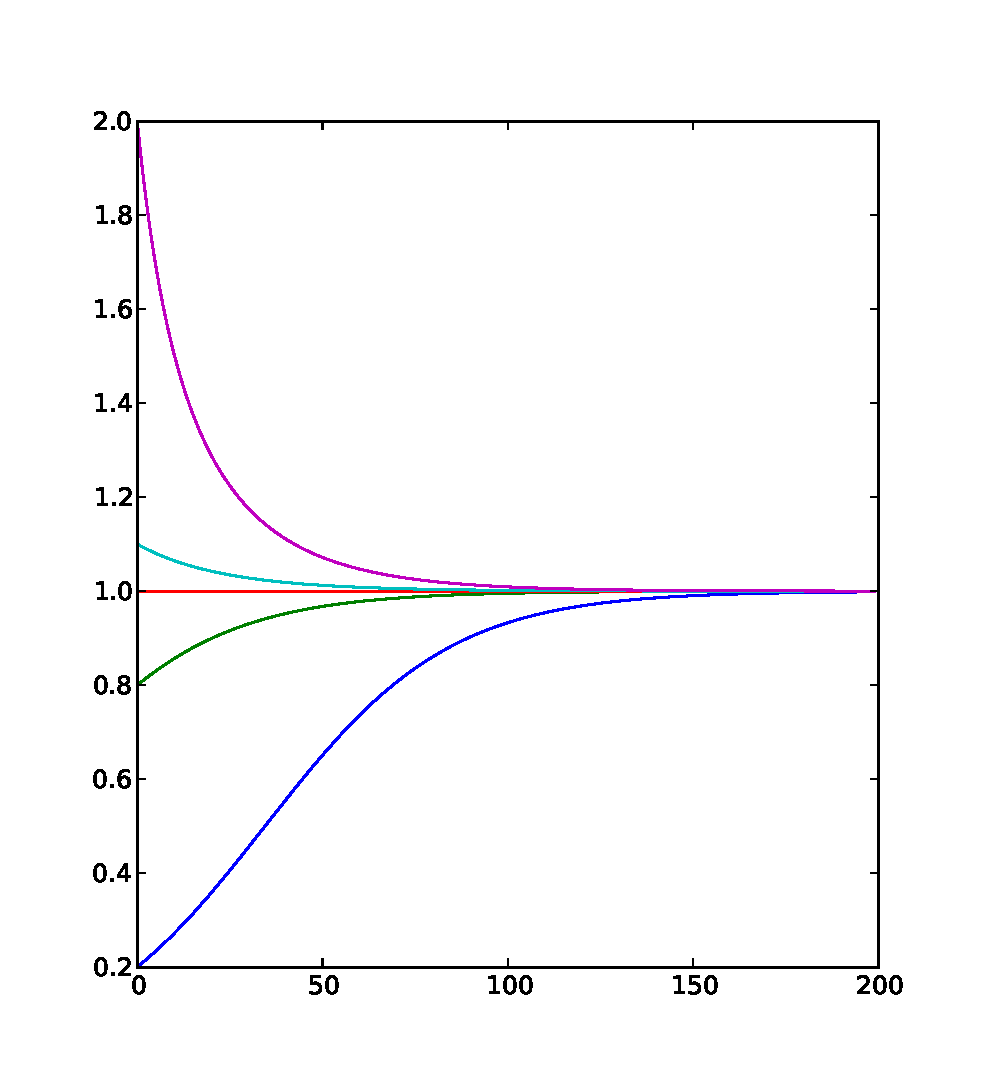
\includegraphics[width=0.75\textwidth]{logistic_diffeq_mu4_varyingx0}
    % for x in (2.0, 1.1, 1.0, 0.8, 0.3):
    %   res = rk4_1D(logistic, x, 2.0, 0.01, (4))
    %   plot(sp.linspace(0,2,201), res)
    % xlim([0,2]); ylim([0,2.01]); xticks(fontsize=24); yticks(fontsize=24)
    % xlabel(r't (time)', fontsize=26); ylabel(r'x(t)', fontsize=26)
  \end{center}
  \caption{
    Plot of equation \pref{eqn:ldesoln} with $\mu = 4$ and various initial values. 
  Regardless of the initial value, $x(t)$ converges to $1$.
}
  \label{fig:lde1}
\end{figure}
We first study the exact solution \pref{eqn:ldesoln}.
If $\mu > 0$, then $e^{\mu t} \to \infty$ as $t \to \infty$, so regardless of the initial value, $x(t)$ converges to the stable state, $x = 1$ (Figure~\ref{fig:lde1}).
%
When $\mu$ is larger, the solution curve converges faster to the stable state (Figure~\ref{fig:lde2}).
As long as $\mu > 0$, however, the asymptotic behavior of the solution does not change.
\begin{figure}[h]
  \begin{center}
    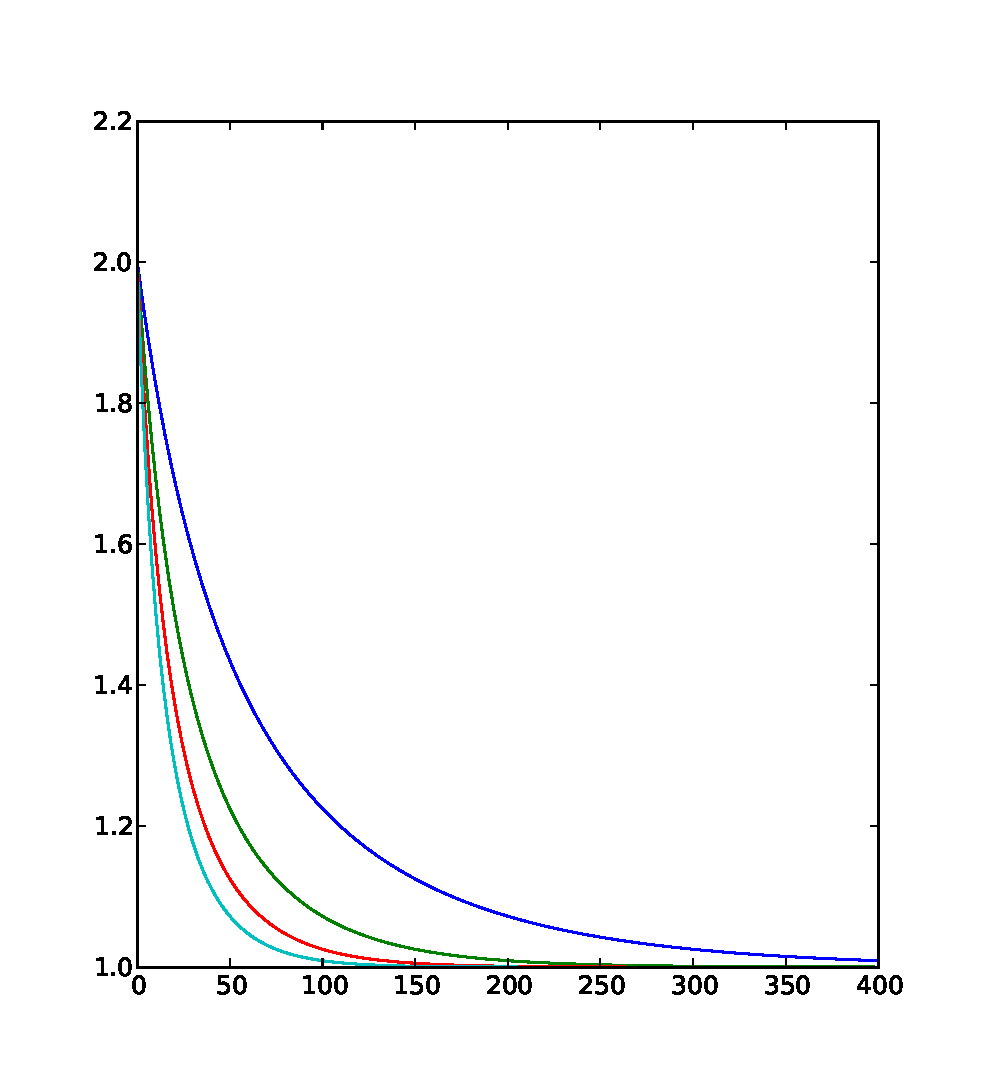
\includegraphics[width=0.75\textwidth]{logistic_diffeq_mu1234_x2}
    % for mu in (1,2,3,4):
    %   res = rk4_1D(logistic, 2.0, 5.0, 0.01, (mu))
    %   plot(sp.linspace(0,5,501), res)
    % xlim([0,5]); ylim([0.99,2.01]); xticks(fontsize=24); yticks(fontsize=24)
    % xlabel(r't (time)', fontsize=26); ylabel(r'x(t)', fontsize=26)
  \end{center}
  \caption{
    Plot of equation \pref{eqn:ldesoln} with $x_0 = 2$ and various $\mu$ ($\mu = 1,2,3,4$).
    As $\mu$ increases, $x(t)$ converges to $1$ faster.
  }
  \label{fig:lde2}
\end{figure}

Next, we study the solution of the discretized model \pref{eqn:logisticsoln} in the same manner.
For $\mu = 1$, solution curves exhibit similar behaviors as the exact solution (Figure~\ref{fig:logistic1-2}).
The stable state has changed to $x = 0$, but for any initial value, the solution curve converges to the stable state.
When $\mu = 2$, the stable state changes to $x = 0.5$.
Thus, we see that \pref{eqn:logisticsoln} does not behave in the exact same manner as \pref{eqn:ldesoln} does.
%\begin{minipage}[t]{0.5\linewidth} <- I could use this.
\begin{figure}[p]
    \centering
    \includegraphics[width=0.75\textwidth]{logistic_map_mu1_varyingx0}
    \includegraphics[width=0.75\textwidth]{logistic_map_mu2_varyingx0}
    % for x in (0.8,0.6,0.4,0.2):
    %   res = IterateList(f, x, 25, (0.25))
    %   plot(res,'o-')
    % xticks(fontsize=24); yticks(fontsize=24)
    % xlabel(r't (time)', fontsize=26); ylabel(r'x(t)', fontsize=26)
    \caption{
      Plot of Equation~\pref{eqn:logisticsoln} for 25 iterations with $\mu = 1$ (top) and $\mu = 2$ (bottom).
      Initial values are $x_0 = 0.2, 0.4, 0.6, 0.8$.
    }
    \label{fig:logistic1-2}
\end{figure}
\begin{figure}[p]
    \centering
    \includegraphics[width=0.75\textwidth]{logistic_map_mu3_varyingx0}
    \includegraphics[width=0.75\textwidth]{logistic_map_mu3_periodic}
    \caption{
      Plot of equation \pref{eqn:logisticsoln} with $\mu = 3$ for 25 (top) and 100 (bottom) iterations.
      Initial values are $x_0 = 0.2, 0.4, 0.6, 0.8$.
    }
    \label{fig:logistic3}
\end{figure}
%%%
\begin{figure}[p]
  \centering
  \includegraphics[width=0.75\textwidth]{logistic_map_mu4_varyingx0}
  \includegraphics[width=0.75\textwidth]{logistic_map_mu4_chaos}
  \caption{
    Plot of equation \pref{eqn:logisticsoln} with $\mu = 4$ for 25 (top) and 100 (bottom) iterations.
    Initial values are $x_0 = 0.2, 0.4, 0.6, 0.8$.
  }
  \label{fig:logistic4}
\end{figure}
%%%
For higher values of $\mu$, the contrast between the two solutions is even more conspicuous.
When $\mu = 3$, the dynamics is almost periodic, but not quite so (Figure~\ref{fig:logistic3}).
The dynamics for $\mu = 4$ is wildly different (Figure~\ref{fig:logistic4}).
Every solution curve moves between 0 and 1, and does not settle down to a periodic behavior.
Moreover, it seems that the solution curves are not even asymptotically periodic.
One might think that this is just a transient behavior, and the solution curves will converge to some values, or at least to some periodic behaviors if we wait long enough.
However, even after 200 or 500 iterations, the logistic map keeps behaving in the same manner (Figure~\ref{fig:chaotic_map}).
This is chaotic.
\begin{figure}[p]
  \centering
  \includegraphics[width=0.75\textwidth]{logistic_map_mu4_x02_200itr}
  \includegraphics[width=0.75\textwidth]{logistic_map_mu4_x02_500itr}
  \caption{
    $\mu = 4$. Initial value $x_0 = 0.2$.
    Top: 200 iterations. Bottom: 500 iterations.
  }
  \label{fig:chaotic_map}
\end{figure}
%%%

This kind of complex behavior arises from the logistic map, one of \textit{the simplest} non-linear equations.
The logistic map for $\mu = 4$ is also known to exhibit \textit{sensitive dependence on initial conditions}, or sensitivity for short.
\index{sensitive dependence on initial conditions}
Sensitivity is considered to be a condition that causes the complicated dynamics of the logistic map.
%Also, we will eventually identify the term ``a chaotic map'' with a mapping that exhibits sensitivity.
To see how sensitivity may bring about complex dynamics, consider the orbits of $x_0 = 0.2$ and a nearby point $y_0 = 0.2 + \epsilon$, where $\epsilon$ is a small positive real number.
Since the two orbits start out close, they remain in the vicinity of each other initially.
However, the two orbits eventually separate from each other, and the distance between them keep growing (Figure~\ref{fig:logistic_sensitivity}).
Thus, a minuscule change in the initial value causes a significant difference in the orbit.
This is not the end of the story.
After the distance between the two reached its maximum, they come closer and closer again, and repeat this process in an aperiodic manner.
\begin{figure}[p]
  \centering
  \includegraphics[width=0.75\textwidth]{logistic_map_sensitivity_x02_mu4}
  %eps = sp.finfo('float').eps
  %plot(IterateList(f, 0.2, 100, (1.0)), 'o-', markersize=8); plot(IterateList(f, 0.2+eps, 100, (1.0)), '>:', markersize=9)
  \includegraphics[width=0.75\textwidth]{logistic_map_sensitivity_x02_mu4_dist}
  % plot(sp.absolute(IterateList(f, 0.2, 100, (1.0)) - IterateList(f, 0.2+eps, 100, (1.0))))
  \caption{
    $\mu = 4$. 100 iterations.
    Initial values: $x_0 = 0.2$ and $y_0 = 0.2 + \epsilon$, where $\epsilon$ is on the order of $10^{-16}$.
    The orbit of $x_0$ is plotted with dashed lines and triangular points.
    The orbit of $y_0$ is plotted with solid lines and circular points.
    The top figure shows the two orbits, and the bottom shows the evolution of distance between them.
  }
  \label{fig:logistic_sensitivity}
\end{figure}
%%%

%In general, we can make a correspondence between continuous and discrete models
%\begin{equation}
% \begin{aligned}
%  \frac{dx(t)}{dt} = G(x(t)) &\quad\mbox{(Continuous)} \\
%  x(t + 1) = F(x(t)) &\quad\mbox{(Discrete)}
%\end{aligned}
%  \label{eqn:intro2}
%\end{equation}
%by regarding the discrete model as an approximation of the continuous model.
%%We can also make the connection by seeing the continuous model as a discrete model where each time step is infinitesimally small.
%The following approximation makes the previous statements more precise:
%\begin{equation*}
%  \frac{dx(t)}{dt} \approx \frac{x(t_0 + (n+1)\Delta t) - x(t_0 + n \Delta t)}{\Delta t}.
%\end{equation*}
%As a result of this approximation, we obtain
%\begin{equation*}
%  F(x(n)) \approx x(n) + \Delta t \cdot G(x(n)).
%\end{equation*}

As it turns out, the logistic map is chaotic in all of the four definitions that we will see.
The logistic map has other interesting properties, as well.
Expositions on the logistic map can be found in many sources.
See \citep{may1, may2, devaney}, for example.
%%%

%\section{Intuitive Notion of Chaos}
%We tend to label a dynamical systems as ``chaotic'' on an intuitive ground, as we saw in defining chaos by fractal dimensions, or by the complicate appearances of attractors.
%If the orbit looks complicated, the system is called chaotic.
%Boris Chirikov and Felix Izrailev, Russian physicists, famously said that ``a strange attractor seems strange only to a stranger.'' \citep{lorentzbook}
%Labeling a system as ``chaotic'' shows our ignorance about the system.
%
%A better way of thinking about chaos should be out there.
%In 1986, the Royal Society held an international conference on chaos and defined ``chaos'' as ``stochastic behavior occurring in a deterministic system.'' \cite{stewart}
%The name is perhaps the cause of these attitudes towards the concept.
%\citet[24]{ueda-abraham}:
%\begin{quotation}
%  As an academic term, I do not find the word 'chaos' very appropriate.
%  But what shall we call it then?
%  My proposal has been ``randomly transitional phenomena''; I will explain this below.
%  The characteristics of chaos in a physical system can be summarized as follows:
%\begin{itemize}
%  \item Random phenomena that occur in deterministic systems.
%  \item Random phenomena whose short-term behavior is predictable.
%  \item Random phenomena whose long-term behavior is unpredictable.
%  \item Although the phenomena are irregular and unpredictable, chaos does have a definite structure.
%\end{itemize}
%  The original meaning of chaos, I feel, is a ``total disorder and ultimate unpredictability.''
%  But as scientific terminology, the word ``chaos'' seems to overemphasize the unpredictability alone.
%  [\ldots]
%  Even so I have to use the word ``chaos'' here. [\ldots]
%  It is a concise expression which has already filtered into people's minds, and therefore I have decided it is rather pointless to resist it.
%\end{quotation}
%%%%
%Ueda's attitude is the one that we adopt in the exposition.
%We do not think that a chaotic map is named so not because it is chaotic in the usual sense.
%We think that finding systems that can be labeled as chaotic should the first step in developing better understandings of those mappings with complicated behaviors.
%
%% Li and Yorke's essay in Chaos Avant-Garde: on how chaos developed over a decade since Poincare (202)
%``He [Robert May] adoped our [Li and Yorke] use of 'chaos' as a mathematical term, and \textit{Period three implies chaos} therefore began to attract considerable worldwide attention by his strong advocacy in talks and papers.
%\ldots
%As use of the word 'chaos' spread, it became a word people loved to hate: they didn't have a better word but didn't like chaos.''
%\citep[205]{ueda-abraham}
%Although there is no universally accepted definition of chaos, most experts would concur that chaos is the {\it aperiodic, long-term behavior of a bounded, deterministic system that exhibits sensitive dependence on initial conditions} (Sprott, p104)
%Our goal is to find the sufficient conditions that give rise to complex orbit structures.
%%%%
%Robert May, a population biologist who is known for studying chaotic behaviors of the logistic map, popularized the term in his articles \citeyearpar{may1,may2}.
%Although the term ``chaos'' is commonly seen in literature nowadays, back when Li and Yorke's paper was being published, ``chaos'' was not an often used word in academic papers.
%Some editors considered the title of their paper to be inappropriate for a language used in an academic article.
%However, some authors admit that the liberal choice of word has to some extent contributed to the popularity that chaos theory currently enjoys \citep[``Exploring Chaos on an Interval'']{ueda-abraham}.
%
%\section{Historical Remarks}
%Chaos is a natural phenoma commonly seen in nonlinear systems in physical sciences.
%Albert Libchaber confirmed chaos via bifurcation in an experiment involving Helium.
%Logistic map is used to model population dynamics.
%Lorentz system was created as a simplified model for atmosphere.
%NH3 lazer is known to show chaotic behavior \citep{kantz-schreiber}.
%B-Z reaction
%Edward Lorentz is often regarded as the first discoverer of chaos.
%\begin{figure}[ht]
%  \centering
%  \includegraphics[scale=0.35]{golden_lorentz_attractor}
%  \caption{The Lorentz Attractor}
%  \label{fig:lorentz}
%\end{figure}
%He found chaotic behaviours through atmospheric simulations using twelve differential equations.
%In his seminal article ``Deterministic Nonperiodic Flow'', Lorentz discusses the chaotic behavior of a system of three differential equations, which were reduced from the original twelve equations.
%Yoshisuke Ueda, though lesser known, was also one of the first scientists to recognize chaotic behaviors.
%In 1961 (a sketch of the ``Japanese Attractor''), while Lorentz's paper was published in 1963.
%David Ruelle, a prominent French chaos researcher, introduced Ueda in \citep{ruelle}.
%
%The reason that I would like to discuss this scientist instead of Lorentz is not because he is the first scientist to see chaos.
%The name ``Japanese Attractor'' was given by David Ruelle.(Les assracteurs etranges; Strange Attractors, 1980)
%% Ueda: 最初はアナログコンピュータが故障したのかと思った。しかしすぐに、いやそんなことはないと悟った (in Chaos Avant-Garde?)
%``I thought vaccum tubes were broken or something---a common issues with computers of those days.'' \citep{lorentzbook} %私はすぐに真空管が弱ったか何かの、よくあるコンピュータトラブルを疑ったが、修理を頼む前に、どこで間違いが起ったかだけでも調べてみることにした
%``As I look back, I feel that after those long exhausting vigils in front of the analog computer, staring atits output, chaos had become a totally natural, everyday phenomenon in my mind.
%People call chaos a new phenomenon, but it has always been around.
%There's nothing new about it---only people did not notice it.''\cite[p.27]{ueda-abraham}
%%「カオス現象は、われわれが、日常、目にしているありふれた実在の自然現象であるにもかかわらず、その概念把握の困難さのために、かっては見過ごされてきた」
%The true value in Ueda's findings lies in its settings.
%While Lorentz's discovery of chaos was through computer simulation of a hypothetical model, Ueda's was through an analog computer, a physical system.
%``analog computeres solve coupled nonlinear equations by mimicking a physical system.
%The error properties of a particular digital integration scheme need not ever be considered.
%Indeed, within the range of accuracy limited by the tolerance of the components, the unsystematic errors caused by the thermal fluctuations and electronic noise in an analog simulation can actually be useful; this is the case, for example, in qualitative studies of chaotic dynamical systems.
%% Crutchfiled, Farmer, Huberman 'Fluctuations and simple chaotic dynamics'
%% Crutchfield, Packard 'Symbolic dynamics of one dimensional maps: Entropies, finite precision, and noise'
%Specifically, these fluctuations obliterate the detailed fine structure found in the mathematical description of chaos and thus effectively mimic the coarse-grained behavior that is observed in actual physical experiments in, for example, convecting fluids or nonlinear electronic circuits.
%''\cite[p.383]{campbell}
%
%\section{Invariants}
%We are looking for invariants of a toplogical dynamical system that characterizes chaos.
%\citet[p.xiii-xv]{schroeder} phrases
%``By symmetry we mean an invariance against change: something stays the same, in spite of some potentially consequential alteration.''
%Motivations to study chaos come not only from the fact that it is a spooky phenomena, but also from practical purposes.
%Chaos time series obtained from a non-linear system could not be analyzed in the same way as linear systems are analyzed.
%Sensitive dependence on initial conditions has an interesting interplay with noises, which are inevitable products in experimental settings.
%\citet[p.51]{kantz-schreiber}:
%\begin{quotation}
%  Noise reduction means that one tries to decompose a time series into two components, one of which supposedly contains the signal and the other one contains random fluctuations.
%  Thus we always assume that the data can be thought of as an additive superposition of two different components which have to be distinguishable by some objective criterion.
%  The classical statistical tool for obtaining this distinction is the power spectrum.
%
%  Random noise has a flat, or at least a broad, spectrum, whereas periodic or quasi-periodic signals have sharp spectral lines.
%  After both components have been identified in the spectrum, a Wiener filter can be used to separate the time series accordingly.
%  This approach fails for deterministic chaotic dynamics because the output of such systems usually leads to broad band spectra itself and thus possesses spectral properties generally attributed to random noise.
%  Even if parts of the spectrum can be clearly associated with the signal, a separation into signal and noise fails for most parts of the frequency domain.
%  Chaotic deterministic systems are of particular interest because the determinism yields an alternative criterion to distinguish the signal and the noise. 
%\end{quotation}
%%%%
%Physicists who are studying systems had to characterize chaotic systems in some way.
%
%We discuss two invariants of dynamical systems that are commonly regarded as signatures of chaos, and de facto \textit{the} definition of chaos: \textit{Lyapunov exponents} and \textit{fractal dimension}.
%The critical feature of the invariants is that they are not sensitive to initial conditions or small perturbations of an orbit, while individual orbits of the system are exponentially
%sensitive to such perturbations. \citep[p.1334]{abarbanel}
%\begin{quote}
%  In the same way power spectrum with a sharp peak characterizes a linear system, invariants such as Lyapunov exponents, fractal dimension, and (KS or topological) entropy characterize nonlinear systems.
%  Each orbit is sensitive to initial conditions; however, these invariants are preserved under small perturbations, which are prevalent in real-life situations.
%\end{quote}
%
%``[B]road (Fourier) power spectrum is a first indication of chaotic behavior, though it alone does not characterize chaos''\citep[p.1338]{abarbanel}
%
%``We say that motion on an attractor is chaotic if it displays sensitive dependence on initial conditions.'' \citep[p.11]{ott1994}
%Two complementary attributes and quantifiers for these attributes sometimes used to define chaos are \citep[p.379]{abarbanel}, %this is not Ott!Abarbanel, then?
%``[\ldots] two key aspects of chaos are the stretching of infinitesimal displacements and the complex orbit structure in the form of a vast variety of possible orbits.'' \citep[p.31]{ott1994}
%\begin{enumerate}
%  \item exponentially sensitive dependence: the largest Lyapunov exponent 
%  \item complex orbit structure: entropy, (metric, topological, or others)
%\end{enumerate}
%
%Although Abarbanel does not include it in his list, an attractor with fractal dimension is a signature of a complex dynamics.
%Note that a treatment of entropy--\textit{topological entropy}, to be specific--will be discussed in Chapter~\ref{chap:entropy} with a more mathematical rigor.
%
%\subsection*{Geometric Definition: Fractal Dimensions}
%Fractals are thought to be closed related to chaos.
%\citet{schroeder} 
%``The word \textit{symmetric} is of ancient Greek parentage and means well-proportioned, well-ordered--certainly nothing even remotely chaotic.
%%Yet, paradoxically, self-similarity, the topic of this tome, alone among all the symmetries gives birth to its very antithesis: \textit{chaos}, a state of utter confusion and disorder.''
%
%Definition of strange attractor\citep[p.131]{ruelle}
%An example where the Hausdorff dimension has an advantage over the box-counting dimension.
%Consider the following infinite sequence:
%\begin{equation*}
%  1, \frac{1}{2}, \frac{1}{3}, \frac{1}{4}, \cdots
%\end{equation*}
%The sequence, when regarded as a set on the real line, has a non-zero box-counting dimension.
%It may be viewed as a dificiency of the box-counting dimension, as one expects that
%a set of discrete points is zero-dimensional.
%The Hausdorff dimension, however, yields zero for this set.
%
%
%(Order and Chaos p103)
%Given that no precise scientific definition exists for the noun ``chaos'' or for the adjective ``chaotic,'' we will consider these words to be synonymous with certain typical properties.
%We will say that a dynamical regime is chaotic if its power spectrum contains a continuous part---a broad band---regardless of the possible presence of peaks.
%Or else we may use the criterion that the autocorrelation function of the time signal has finite support, i.e. that it goes to zero in a finite time.
%In either case, the same concept is involved: the loss of memory of the signal with respect to itself.
%Consequently, knowledge of the state of the system for an arbitrarily long time does not enable us to predict its later evolution.
%Essentially, this means that we are making unpredictability the quality which defines chaos.
%The characterization is pragmatic; it lacks rigor and contains unavoidable ambiguities.
%The boundary separating predictability from unpredictability is unclear, leaving open questions such as:
%- On what time scale must the flow be predictable?
%- How precise must the prediction be?
%- Can we allow a statistical prediction?
%The distinction between the theoretical and practical impossibility of prediction is also problematic.
%But given the current state of knowledge, it would be premature to try to do better.
%
%%%%
%
%
%\subsection*{Lyapunov Exponents In One Dimension}
%The technique of Lyapunov exponents was developed by Alexander M. Lyapunov to study stability of solutions for systems of differential equations.
%Although positive Lyapunov exponent is commonly regarded as the definition of chaos \citep{kantz-schreiber} in physics, we do not discuss it in detail, since the Lyapunov exponent is only defined for differentiable mappings.
%Since our focus is on topolgical dynamics, we do not go into a great detail explaning Lyapunov exponent.
%Lyapunov exponent, however, gives some mathematical content to the word sensitive dependence on initial conditions, and also illustrates the idea of invariants.
%We rather informally define the Lyapunov exponent below to give the reader 
%%Lyapunov exponents are sometimes called characteristic exponents.
%%Also, \citet{young} gave a lower bound of the Hausdorff dimension in terms of the Lyapunov numbers, so the geometry of a dynamical system is not unrelated to sensitive dependence on initial conditions.
%\begin{definition}
%  (Lyapunov exponent)
%  Let $F: \R \to \R$ be a differentiable mapping, and $x_0 \in \R$.
%  We define the Lyapunov exponent of $O(x_0)$.
%  We use the following notation $x_i \ceq \itr{F}{i}(x_0)$.
%  Define Jacobian matrices
%  \begin{equation*}
%    A_0 \ceq F'(x_0),
%    \; A_1 \ceq F'(x_1),
%    \; \ldots,
%    \; A_n \ceq F'(x_n).
%  \end{equation*}
%  Then, denote the spectral radii (i.e. the maximum of the absolute values of eigenvalues) of $A_i$ by $\rho_i(x_0)$.
%  Then the Lyapunov number $N(x_0)$ of $O(x_0)$ is defined as 
%  \begin{equation*}
%    N(x_0) = \lim\limits_{n \to \infty} (\rho_n(x_0))^{1/n}.
%  \end{equation*}
%  Then, we define the Lyapunov exponent to be the log of the Lyapunov number.
%  \begin{equation*}
%    \Lambda(x_1) = \log N(x_1).
%  \end{equation*}
%  In particular,
%  \begin{equation*}
%    \Lambda(x_1) = \lim\limits_{n \to \infty} \paren{\log\abs{F'(x_n)} + \log\abs{F'(x_{n-1})} + \cdots + \log\abs{F'(x_1)}}
%  \end{equation*}
%  \index{Lyapunov number}
%\end{definition}
%%(Lyapunov exponent is computationally preferable to the Lyapunov number.)
%%It can be shown that the Lyapunov exponent of a map is (almost everywhere) equivalent to the Lyapunov exponent of any orbit of a map (Lyapunov exponent is independent of orbit).
%\begin{proposition}
%  Suppose $h'(x) \neq 0$ and
%  \begin{equation*}
%    \lim\limits_{n\to \infty} \frac{\log\abs{h'(x_n)}}{n} = 0.
%  \end{equation*}
%  Then, the Lyapunov numbers of one-dimensional dynamical systems that are conjugate is the same 
%  \label{prop:lyap-conj}
%  \begin{proof}
%    \begin{equation*}
%      h'(x_{n+1})F'(x_n)\ldots F'(x_1) = G'(y_n)\ldots G'(y_1)h'(x_1).
%    \end{equation*}
%    Then 
%    \begin{align*}
%      \Lambda(x_1) &= \lim\limits_{n\to \infty} \frac{1}{n}\paren{\log\abs{F'(x_n)} + \cdots + \log\abs{F'(x_n)} } \\
%      &= \lim\limits_{n\to \infty} \frac{1}{n}\left(\log\abs{F'(x_n)} + \cdots + \log\abs{F'(x_n)} + \log\abs{h'(x_{n+1})}\right) \\
%      &= \lim\limits_{n\to \infty} \frac{1}{n} \paren{ \log\abs{G'(x_n)} + \cdots + \log\abs{G'(x_n)} + \log\abs{h'(x_1)} } \\
%      &= \lim\limits_{n\to \infty} \frac{1}{n} \paren{ \log\abs{G'(x_n)} + \cdots + \log\abs{G'(x_n)} } \\
%      &= \Lambda(y_1),
%    \end{align*} 
%    as desired.
%  \end{proof}
%\end{proposition}
%%%%
%Lyapunov exponent is a convenient method of seeing if a system is sensitive to initial conditions, and it is widely used in experimental settings.
%Even so, Lyapunov exponent should be treated with some care, as the next example suggests.
%\begin{example}
%  \citep{wiggins}
%  Consider the following vector field:
%  \begin{equation*}
%    \dot{x} = ax,
%  \end{equation*}
%  where $x \in \R$, and $a \in \R$ is a constant.
%  The Lyapunov exponent of each orbit is $a > 0$.
%\end{example}
%%
%
%\section{Outline Of The Exposition}
%In Chapters~\ref{chap:devaney} and \ref{chap:liyorke}, we will see the two most often talked about definitions of chaos.
%In Chapter~\ref{chap:symbolic}, symbolic dynamcis.
%In Chapter~\ref{chap:entropy}, topological entropy.
%In chapter~\ref{chap:billiards}, we present a system that seems to be chaotic.
%
%Also, we should note that, though chaotic dynamical systems is a large field, the field of dynamical systems in general is even larger.
%In dynamical systems, given a system, one asks whether the system is stable or has periodic elements, and so on.
%Asking whether a system is chaotic, is, in some sense, a sloppy way of thinking about systems.
%To label a system as ``chaotic'' and avoid asking further questions is to neglect the intricacies that a system may have.
%Characterization of a system as a chaotic system should be a beginning of the study of systems.
%That is, chaotic systems may perhaps be further divided into different categories, and could be understood better.
%\citet{devaney}, for example, discusses different ``routes'' to chaos.
%As we will see, there are systems that are chaotic in some sense but not so in others.
%I mentioned at the beginning that the goal of this exposition is to find an appropriate definition of chaos.
%However, it may be possible that different deterministic systems are unpredictable in different senses.
%I hope to 
%
%\bibliographystyle{../../bibliography/pjgsm}
%\bibliography{../../bibliography/thesis}
%
\end{document}
